\chapter{Methodology and Project Management}

When managing the development of a project, there are several approaches one can take when planning the development lifecycle \parencite{shylesh2017study}; the three main approaches for any project are sequential (linear), incremental, and iterative (non-linear) phases \parencite{akinsola2020comparative}, which methodology is best suited depends on the nature of the application. The nature of this project involved one developer with evolving requirements, adaptable features, and unforeseen management issues, therefore the following methodologies were explored and appropriately chosen.

The planning and development carried throughout this project were based on an agile methodology model designed for specific and individual use. This section discusses how to differentiate between the most appropriate and applicable methodology, to which will establish the final selected software development lifecycle model (SDLC). The scope for this project can be displayed as such:

\begin{figure}[H]
    \centering
    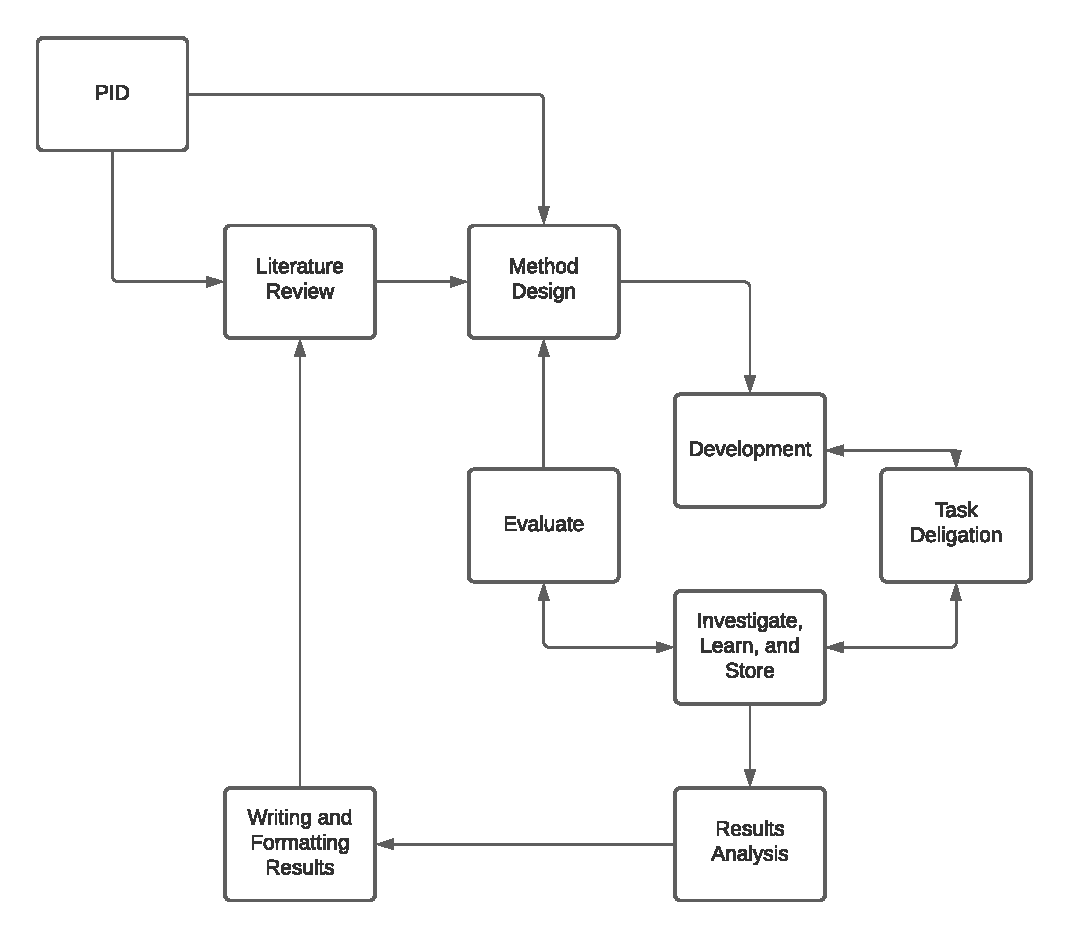
\includegraphics[width=\textwidth]{figures/chapter-3/ProjectOverviewFlowChart.pdf}
    \caption[Overview of Project Workflow]{Overview of my project from start to finish
    \label{fig:ProjectWorkflow}}
\end{figure}

As seen in \autoref{fig:ProjectWorkflow}, this project follows an iterative process with included circular motion for data validation and section corroboration. Due to this nature, it seems a hybrid SDLC Model is best suited for this project; the apparent combination of methodologies allows for aspects from both strict Test-Driven Development and Rapid Application Development without the inclusion of their inherent disadvantages.

Whilst the original commencement plan for this project was entirely constructed on the Waterfall Model as depicted in the supplied Gantt Chart within the PID document, this however, was not a sufficient process mainly due to time constraints, thus the Waterfall Model structure was partly ignored to allow for improved efficiency requirements and minor tweaks to previously stated tasks. These tweaks are outlined in the final chosen (adapted) model.

\section{Methodologies}

This project uses two SDLC’s, one for the project in its entirety and one for development.

\subsection{Data Mining}

This project’s primary objective is text classification which focuses on predictive aspects of NLP, data mining and analytics are inherently used in machine-learning and natural language processing as for a model to be predictive there must be a history of data to be analysed, this project uses openly sourced student feedback from Kaggle to achieve clean and rich data without breaching ethical concerns.

Big datasets are becoming widely used for research and data-mining techniques aid development as they ensure the correct dataset is being used, appropriate data must be used for the applied techniques and data manipulation because inappropriate data could lead to inaccurate or misleading results. It is essential that the use of data is appropriate for the proposed machine learning model, in the scope of this project it is student feedback being mined and analysed through a predictive model.

\subsection{Data Analytics}

Data analytics is a necessary topic for NLP to achieve the desired outcome; within this project, the outline goal is to be able identify lexical trends by analysis a given dataset to answer predict questions and potentially speculate a topical conclusion, i.e., a certain student is content in their feedback. This data-driven decisions and outcomes are only possible from analysing existing datasets and their inherent meaning(s); data analytics is a broad area within machine learning and this project concentrates on descriptive analysis and predictive analysis. The data analytics being performed on the chosen datasets are predominately for pattern recognition and accuracy improvements.

\subsection{Developmental Flowchart}

The elected methodology for this project is a bespoke hybrid model that includes features from sections 3.2.1, 3.2.2, and 3.2.3 to reap the benefits from each stated methodology whilst minimising the drawbacks. The proposed model is a specific draft construction with the focus on machine learning projects, it is appropriately titled Machine Learning Development Lifecycle and is its own SDLC. The proposed methodology can be displayed as a flowchart:

\begin{figure}[H]
    \centering
    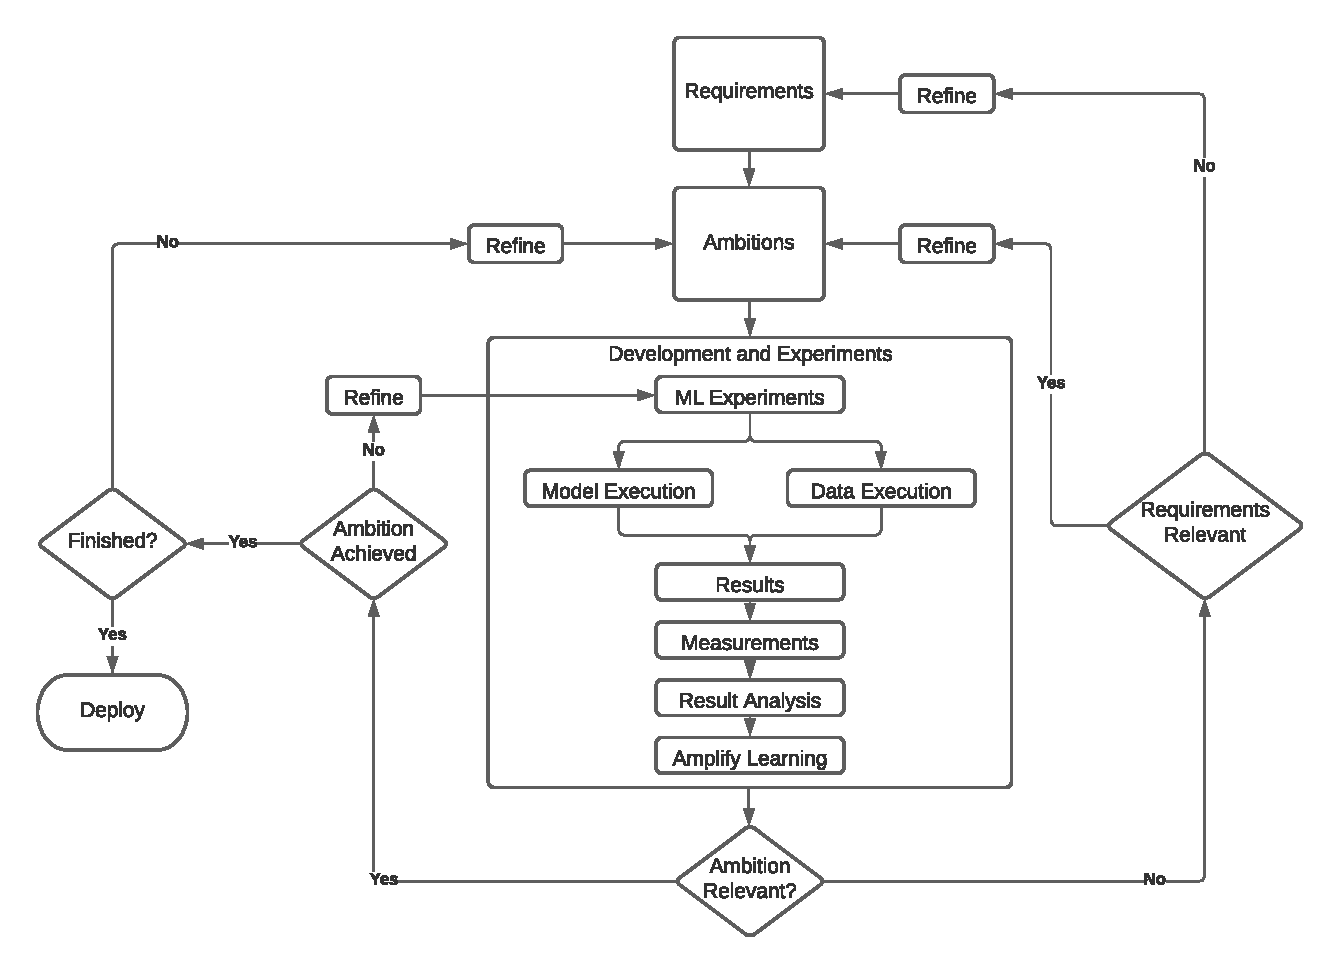
\includegraphics[width=\textwidth]{figures/chapter-3/MLDC.pdf}
    \caption[Machine Learning Development Lifecycle]{Workflow for the development of my project.
    \label{fig:MLDC}}
\end{figure}

The proposed methodology includes an Agile and Iterative core, the project requirements are directly transposed into the ML ambitions, the ML ambitions are obtained with the guidance of its experiments. This approach allows for deferred commitment with scope and requirements, code quality and coverage whilst achieving a quick artifact delivery \parencite{pinhasi2021mldc}.

\subsection{Elected SDLC}

This project strictly follows the Cross Industry Process for Data Mining model, widely known as CRISP-DM; when executing the development of a machine learning based project, there are several prefacing steps such as planning, organisation, and implementation, currently there is no standard model to efficiently carry out the development of such a project and this is where the CRISP---DM model is useful. It aims to intersect personal skills and knowledge into an effective and effective process \parencite{wirth2000crisp}. The proposed workflow can be displayed within a model such that:

\begin{figure}[H]
    \centering
    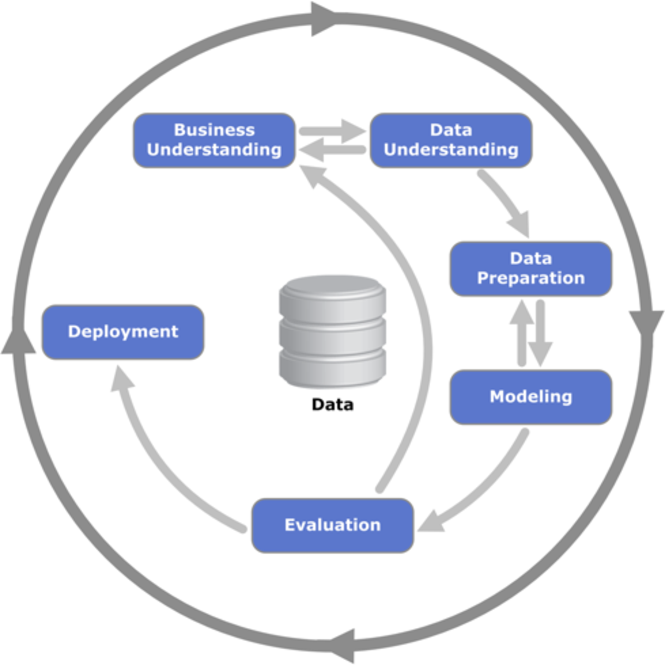
\includegraphics[width=\textwidth]{figures/chapter-3/CRISP-DM1.pdf}
    \caption[CRISP-DM Lifecycle]{The CRISP-DM Software Development Lifecycle \parencite{jenson2012crisp}.
    \label{fig:CRISP-DM}}
\end{figure}

This methodology can be described as a hierarchical process model as there is an apparent level of abstraction, being described as: phases, generic tasks, specialised tasks, and process instances \parencite{wirth2000crisp}. This process is beneficial as it can be applied to this project, each section is broken down into its respected hierarchy and labelled appropriately which is then handled in development, it allows for stable agile development as the developer can refine requirements or datasets as the project goes on, however acknowledging potential unforeseen aspects.

The process model can be deconstructed into six specific categories or phases (\autoref{fig:CRISP-DM}):

\begin{itemize}
    \item \textbf{\textit{Business Understanding}}: rather than business understanding, the context for this project is the project scope itself, the developer needs to understand the context of the problem.
    \item \textbf{\textit{Data Understanding}}: understanding the initial data collected to identify data quality and detect potential insights.
    \item \textbf{\textit{Data Preparation}}: once the initial data is collected and analysed, it will need to be prepared to construct a finalised usable dataset for the model to be parsed.
    \item \textbf{\textit{Modelling}}: this phase deals with how the data is parsed into the model after applying the intended ML techniques, this is very similar to preparation phase.
    \item \textbf{\textit{Evaluation}}: once the desired models have been constructed and the data has been parsed, it will need a quality check to ensure analysis is correct before deployment.
    \item \textbf{\textit{Deployment}}: the requirements have been met by the developer and the model yield appropriate results, the model can be deployed to an appropriate environment.
\end{itemize}

As data mining is not a standard domain which can produce varied results depending on how the project is structured and outlined, the need for a standard framework was apparent for this project. There is not reject reasoning behind this selected SDLC as the approach aims to improve accuracy, efficiency, and effectiveness of data mining applications.

\section{Project Management}

\subsection{Development Management}

The source code to this project was decided to be monitored via a GIT repository stored on GitHub; the use of version control for a machine-learning based project is especially helpful as you can backtrack certain functions that outperform changes without affecting the entire stack. The choice to use GIT opposed to a local project had several factors, such as:

\begin{itemize}
    \item Version control
    \item Track bugs
    \item Back-Up complete
    \item Branches for different features
    \item Testing purposes
    \item Source Code sharing
        \begin{itemize}
            \item Developer to supervisor
            \item Developer to developer systems
        \end{itemize}
\end{itemize}

GitHub was the chosen hosting platform due to industry standard and familiarity to both the developer and project supervisor, however, other GIT based hosting platforms such as GitLab or BitBucket do exist that satisfy the same project requirements.

\subsection{Task Management}

Delegation of project tasks evolved over the course of completion; mentally keeping track of project TODOs became mentally taxing, thus a formal system for task delegation was implemented. As this project was completed by a sole developer, that immediately ruled out the use of a SCRUM based project board as team roles were not necessary, therefore, the “easy-to-adopt” KANBAN method was implemented, which by itself is also justification for a LEAN based SDLC model. KANBAN is a solution in which eases aspects of project design, management, improvement flow and situational knowledge and awareness by visualising (a simplified) “TODO”, “DOING”, and “DONE” categories. This in turn balances work demands compared to work capacity.

% TODO add figures for kanban boards

This project uses two KANBAN applications, separated by general delegation and development delegation, to oversee metrics such as developer velocity, lead and time cycle, and actionable agile metrics, a Trello Board was implemented that included all tasks related to this project and report. In addition, a GitKraken Board was used for development related tasks such as feature ideas and bugs, these two boards were synced for a complete overview of tasks on Trello to capture the project’s work-in-progress (WIP) limits.

% TODO add figures for trello and gitkracken

\subsection{Time Management}

Within the Project-initiation Document (PID) in Appendix A, a Gantt Chart is supplied detailing the expected timeline this project will follow. However, it was subject to change and adaptions due to unforeseen circumstances, the below is a Gantt Chart detailing an accurate time-frame which was created nearer project end:

\begin{figure}[H]
    \centering
    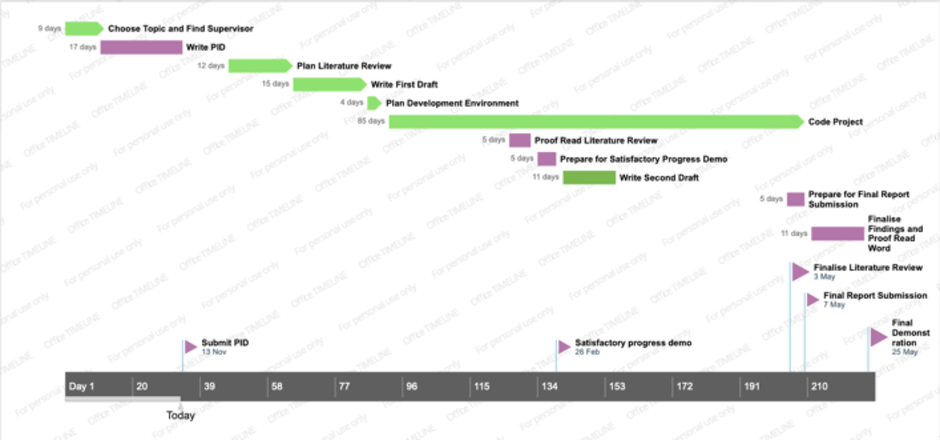
\includegraphics[width=\textwidth]{figures/chapter-3/ProjectGanttChart.pdf}
    \caption[Project Gantt Chart]{Project Gantt Chart.
    \label{fig:ProjectGanttChart}}
\end{figure}
